
\documentclass[letterpaper,hide notes,xcolor={table,svgnames},pdftex,10pt]{beamer}
\def\showexamples{t}


%\usepackage[svgnames]{xcolor}

%% Demo talk
%\documentclass[letterpaper,notes=show]{beamer}

\usecolortheme{crane}
\setbeamertemplate{navigation symbols}{}

\usetheme{PlamPittsburgh}
%\usetheme{Frankfurt}

%\usepackage{tipa}

\usepackage{hyperref}
\usepackage{graphicx,xspace}
\usepackage[normalem]{ulem}
\usepackage{multicol}
\usepackage{amsmath,amssymb,amsthm,graphicx,xspace}
\newcommand\SF[1]{$\bigstar$\footnote{SF: #1}}

\usepackage[default]{sourcesanspro}
\usepackage[T1]{fontenc}
\usepackage[scaled]{beramono}
\usepackage{tikzpagenodes}

\newcounter{tmpnumSlide}
\newcounter{tmpnumNote}


% old question code
%\newcommand\question[1]{{$\bigstar$ \small \onlySlide{2}{#1}}}
% \newcommand\nquestion[1]{\ifdefined \presentationonly \textcircled{?} \fi \note{\par{\Large \textbf{?}} #1}}
% \newcommand\nanswer[1]{\note{\par{\Large \textbf{A}} #1}}


 \newcommand\mnote[1]{%
   \addtocounter{tmpnumSlide}{1}
   \ifdefined\showcues {~\tiny\fbox{\arabic{tmpnumSlide}}}\fi
   \note{\setlength{\parskip}{1ex}\addtocounter{tmpnumNote}{1}\textbf{\Large \arabic{tmpnumNote}:} {#1\par}}}

\newcommand\mmnote[1]{\note{\setlength{\parskip}{1ex}#1\par}}

%\newcommand\mnote[2][]{\ifdefined\handoutwithnotes {~\tiny\fbox{#1}}\fi
% \note{\setlength{\parskip}{1ex}\textbf{\Large #1:} #2\par}}

%\newcommand\mnote[2][]{{\tiny\fbox{#1}} \note{\setlength{\parskip}{1ex}\textbf{\Large #1:} #2\par}}

\newcommand\mquestion[2]{{~\color{red}\fbox{?}}\note{\setlength{\parskip}{1ex}\par{\Large \textbf{?}} #1} \note{\setlength{\parskip}{1ex}\par{\Large \textbf{A}} #2\par}\ifdefined \presentationonly \pause \fi}

\newcommand\blackboard[1]{%
\ifdefined   \showblackboard
  {#1}
  \else {\begin{center} \fbox{\colorbox{blue!30}{%
         \begin{minipage}{.95\linewidth}%
           \hspace{\stretch{1}} Some space intentionally left blank; done at the blackboard.%
         \end{minipage}}}\end{center}}%
         \fi%
}



%\newcommand\q{\tikz \node[thick,color=black,shape=circle]{?};}
%\newcommand\q{\ifdefined \presentationonly \textcircled{?} \fi}

\usepackage{listings}
\lstset{basicstyle=\footnotesize\ttfamily,
	breaklines=true,
	aboveskip=15pt,
  	belowskip=15pt,
	frame=lines,
	numbers=left, basicstyle=\scriptsize, numberstyle=\tiny, stepnumber=0, numbersep=2pt
}

\usepackage{siunitx}
\newcommand\sius[1]{\num[group-separator = {,}]{#1}\si{\micro\second}}
\newcommand\sims[1]{\num[group-separator = {,}]{#1}\si{\milli\second}}
\newcommand\sins[1]{\num[group-separator = {,}]{#1}\si{\nano\second}}
\sisetup{group-separator = {,}, group-digits = true}

%% -------------------- tikz --------------------
\usepackage{tikz}
\usetikzlibrary{positioning}
\usetikzlibrary{arrows,backgrounds,automata,decorations.shapes,decorations.pathmorphing,decorations.markings,decorations.text}

\tikzstyle{place}=[circle,draw=blue!50,fill=blue!20,thick, inner sep=0pt,minimum size=6mm]
\tikzstyle{transition}=[rectangle,draw=black!50,fill=black!20,thick, inner sep=0pt,minimum size=4mm]

\tikzstyle{block}=[rectangle,draw=black, thick, inner sep=5pt]
\tikzstyle{bullet}=[circle,draw=black, fill=black, thin, inner sep=2pt]

\tikzstyle{pre}=[<-,shorten <=1pt,>=stealth',semithick]
\tikzstyle{post}=[->,shorten >=1pt,>=stealth',semithick]
\tikzstyle{bi}=[<->,shorten >=1pt,shorten <=1pt, >=stealth',semithick]

\tikzstyle{mut}=[-,>=stealth',semithick]

\tikzstyle{treereset}=[dashed,->, shorten >=1pt,>=stealth',thin]

\usepackage{ifmtarg}
\usepackage{xifthen}
\makeatletter
% new counter to now which frame it is within the sequence
\newcounter{multiframecounter}
% initialize buffer for previously used frame title
\gdef\lastframetitle{\textit{undefined}}
% new environment for a multi-frame
\newenvironment{multiframe}[1][]{%
\ifthenelse{\isempty{#1}}{%
% if no frame title was set via optional parameter,
% only increase sequence counter by 1
\addtocounter{multiframecounter}{1}%
}{%
% new frame title has been provided, thus
% reset sequence counter to 1 and buffer frame title for later use
\setcounter{multiframecounter}{1}%
\gdef\lastframetitle{#1}%
}%
% start conventional frame environment and
% automatically set frame title followed by sequence counter
\begin{frame}%
\frametitle{\lastframetitle~{\normalfont(\arabic{multiframecounter})}}%
}{%
\end{frame}%
}
\makeatother

\makeatletter
\newdimen\tu@tmpa%
\newdimen\ydiffl%
\newdimen\xdiffl%
\newcommand\ydiff[2]{%
    \coordinate (tmpnamea) at (#1);%
    \coordinate (tmpnameb) at (#2);%
    \pgfextracty{\tu@tmpa}{\pgfpointanchor{tmpnamea}{center}}%
    \pgfextracty{\ydiffl}{\pgfpointanchor{tmpnameb}{center}}%
    \advance\ydiffl by -\tu@tmpa%
}
\newcommand\xdiff[2]{%
    \coordinate (tmpnamea) at (#1);%
    \coordinate (tmpnameb) at (#2);%
    \pgfextractx{\tu@tmpa}{\pgfpointanchor{tmpnamea}{center}}%
    \pgfextractx{\xdiffl}{\pgfpointanchor{tmpnameb}{center}}%
    \advance\xdiffl by -\tu@tmpa%
}
\makeatother
\newcommand{\copyrightbox}[3][r]{%
\begin{tikzpicture}%
\node[inner sep=0pt,minimum size=2em](ciimage){#2};
\usefont{OT1}{phv}{n}{n}\fontsize{4}{4}\selectfont
\ydiff{ciimage.south}{ciimage.north}
\xdiff{ciimage.west}{ciimage.east}
\ifthenelse{\equal{#1}{r}}{%
\node[inner sep=0pt,right=1ex of ciimage.south east,anchor=north west,rotate=90]%
{\raggedleft\color{black!50}\parbox{\the\ydiffl}{\raggedright{}#3}};%
}{%
\ifthenelse{\equal{#1}{l}}{%
\node[inner sep=0pt,right=1ex of ciimage.south west,anchor=south west,rotate=90]%
{\raggedleft\color{black!50}\parbox{\the\ydiffl}{\raggedright{}#3}};%
}{%
\node[inner sep=0pt,below=1ex of ciimage.south west,anchor=north west]%
{\raggedleft\color{black!50}\parbox{\the\xdiffl}{\raggedright{}#3}};%
}
}
\end{tikzpicture}
}


%% --------------------

%\usepackage[excludeor]{everyhook}
%\PushPreHook{par}{\setbox0=\lastbox\llap{MUH}}\box0}

%\vspace*{\stretch{1}

%\setbox0=\lastbox \llap{\textbullet\enskip}\box0}

\setlength{\parskip}{\fill}

\newcommand\noskips{\setlength{\parskip}{1ex}}
\newcommand\doskips{\setlength{\parskip}{\fill}}

\newcommand\xx{\par\vspace*{\stretch{1}}\par}
\newcommand\xxs{\par\vspace*{2ex}\par}
\newcommand\tuple[1]{\langle #1 \rangle}
\newcommand\code[1]{{\sf \footnotesize #1}}
\newcommand\ex[1]{\uline{Example:} \ifdefined \presentationonly \pause \fi
  \ifdefined\showexamples#1\xspace\else{\uline{\hspace*{2cm}}}\fi}

\newcommand\ceil[1]{\lceil #1 \rceil}


\AtBeginSection[]
{
   \begin{frame}
       \frametitle{Outline}
       \tableofcontents[currentsection]
   \end{frame}
}



\pgfdeclarelayer{edgelayer}
\pgfdeclarelayer{nodelayer}
\pgfsetlayers{edgelayer,nodelayer,main}

\tikzstyle{none}=[inner sep=0pt]
\tikzstyle{rn}=[circle,fill=Red,draw=Black,line width=0.8 pt]
\tikzstyle{gn}=[circle,fill=Lime,draw=Black,line width=0.8 pt]
\tikzstyle{yn}=[circle,fill=Yellow,draw=Black,line width=0.8 pt]
\tikzstyle{empty}=[circle,fill=White,draw=Black]
\tikzstyle{bw} = [rectangle, draw, fill=blue!20, 
    text width=4em, text centered, rounded corners, minimum height=2em]
    
    \newcommand{\CcNote}[1]{% longname
	This work is licensed under the \textit{Creative Commons #1 3.0 License}.%
}
\newcommand{\CcImageBy}[1]{%
	\includegraphics[scale=#1]{creative_commons/cc_by_30.pdf}%
}
\newcommand{\CcImageSa}[1]{%
	\includegraphics[scale=#1]{creative_commons/cc_sa_30.pdf}%
}
\newcommand{\CcImageNc}[1]{%
	\includegraphics[scale=#1]{creative_commons/cc_nc_30.pdf}%
}
\newcommand{\CcGroupBySa}[2]{% zoom, gap
	\CcImageBy{#1}\hspace*{#2}\CcImageNc{#1}\hspace*{#2}\CcImageSa{#1}%
}
\newcommand{\CcLongnameByNcSa}{Attribution-NonCommercial-ShareAlike}

\newenvironment{changemargin}[1]{% 
  \begin{list}{}{% 
    \setlength{\topsep}{0pt}% 
    \setlength{\leftmargin}{#1}% 
    \setlength{\rightmargin}{1em}
    \setlength{\listparindent}{\parindent}% 
    \setlength{\itemindent}{\parindent}% 
    \setlength{\parsep}{\parskip}% 
  }% 
  \item[]}{\end{list}} 



\title{Lecture 1 --- Programming for Performance}

\author{Jeff Zarnett \& Patrick Lam \\ \small \texttt{jzarnett@uwaterloo.ca, patrick.lam@uwaterloo.ca}}
\institute{Department of Electrical and Computer Engineering \\
  University of Waterloo}
\date{\today}


\begin{document}

\begin{frame}
  \titlepage

 \end{frame}

\begin{frame}
\frametitle{Lucas, SE2015}

\begin{center}
\includegraphics[width=.9\textwidth]{images/lucas_waterton.jpg}
\end{center}
\end{frame}

\begin{frame}
\frametitle{The Continental Divide Trail}
\begin{center}
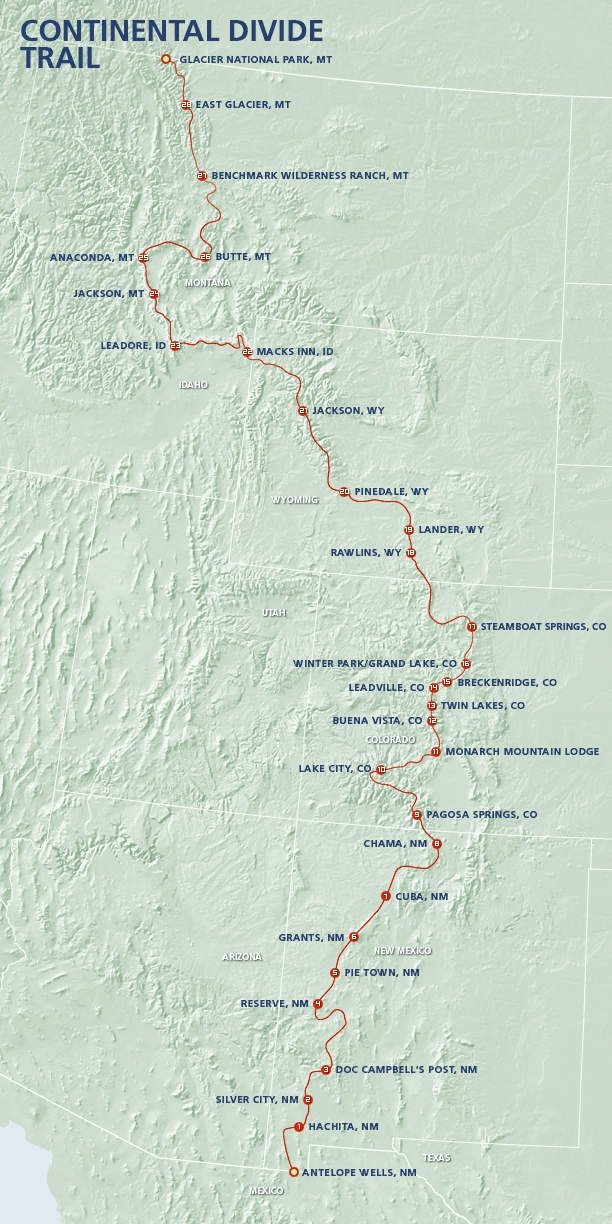
\includegraphics[width=.3\textwidth]{images/cdt.png}
~\\
3000 miles, 5 months.\\
How to do faster?
\end{center}
\end{frame}

\begin{frame}
\frametitle{Course Syllabus}
\Large
As our first order of business, \\
let's go over the course syllabus.

\end{frame}

\begin{frame}
\frametitle{Collaborative Course}
\Large

The source material for the ECE~459 notes~\&~slides is available via Github. 

If you find an error in the notes/slides, \\
or have an improvement, go to \url{https://github.com/jzarnett/ece459} and open an issue. 

You can submit a pull request (changes) for me to look at and incorporate!

\end{frame}



\begin{frame}
\frametitle{Performance!}
\large

I'm certain you know what ``programming'' means. \\
But define ``performance''. 

A: Making a program ``fast''. 

Alright\ldots\\ 
\qquad but what does it mean for a program to be fast?

\end{frame}

\begin{frame}
\frametitle{What is Fast?}

\begin{changemargin}{-1cm}
\begin{center}
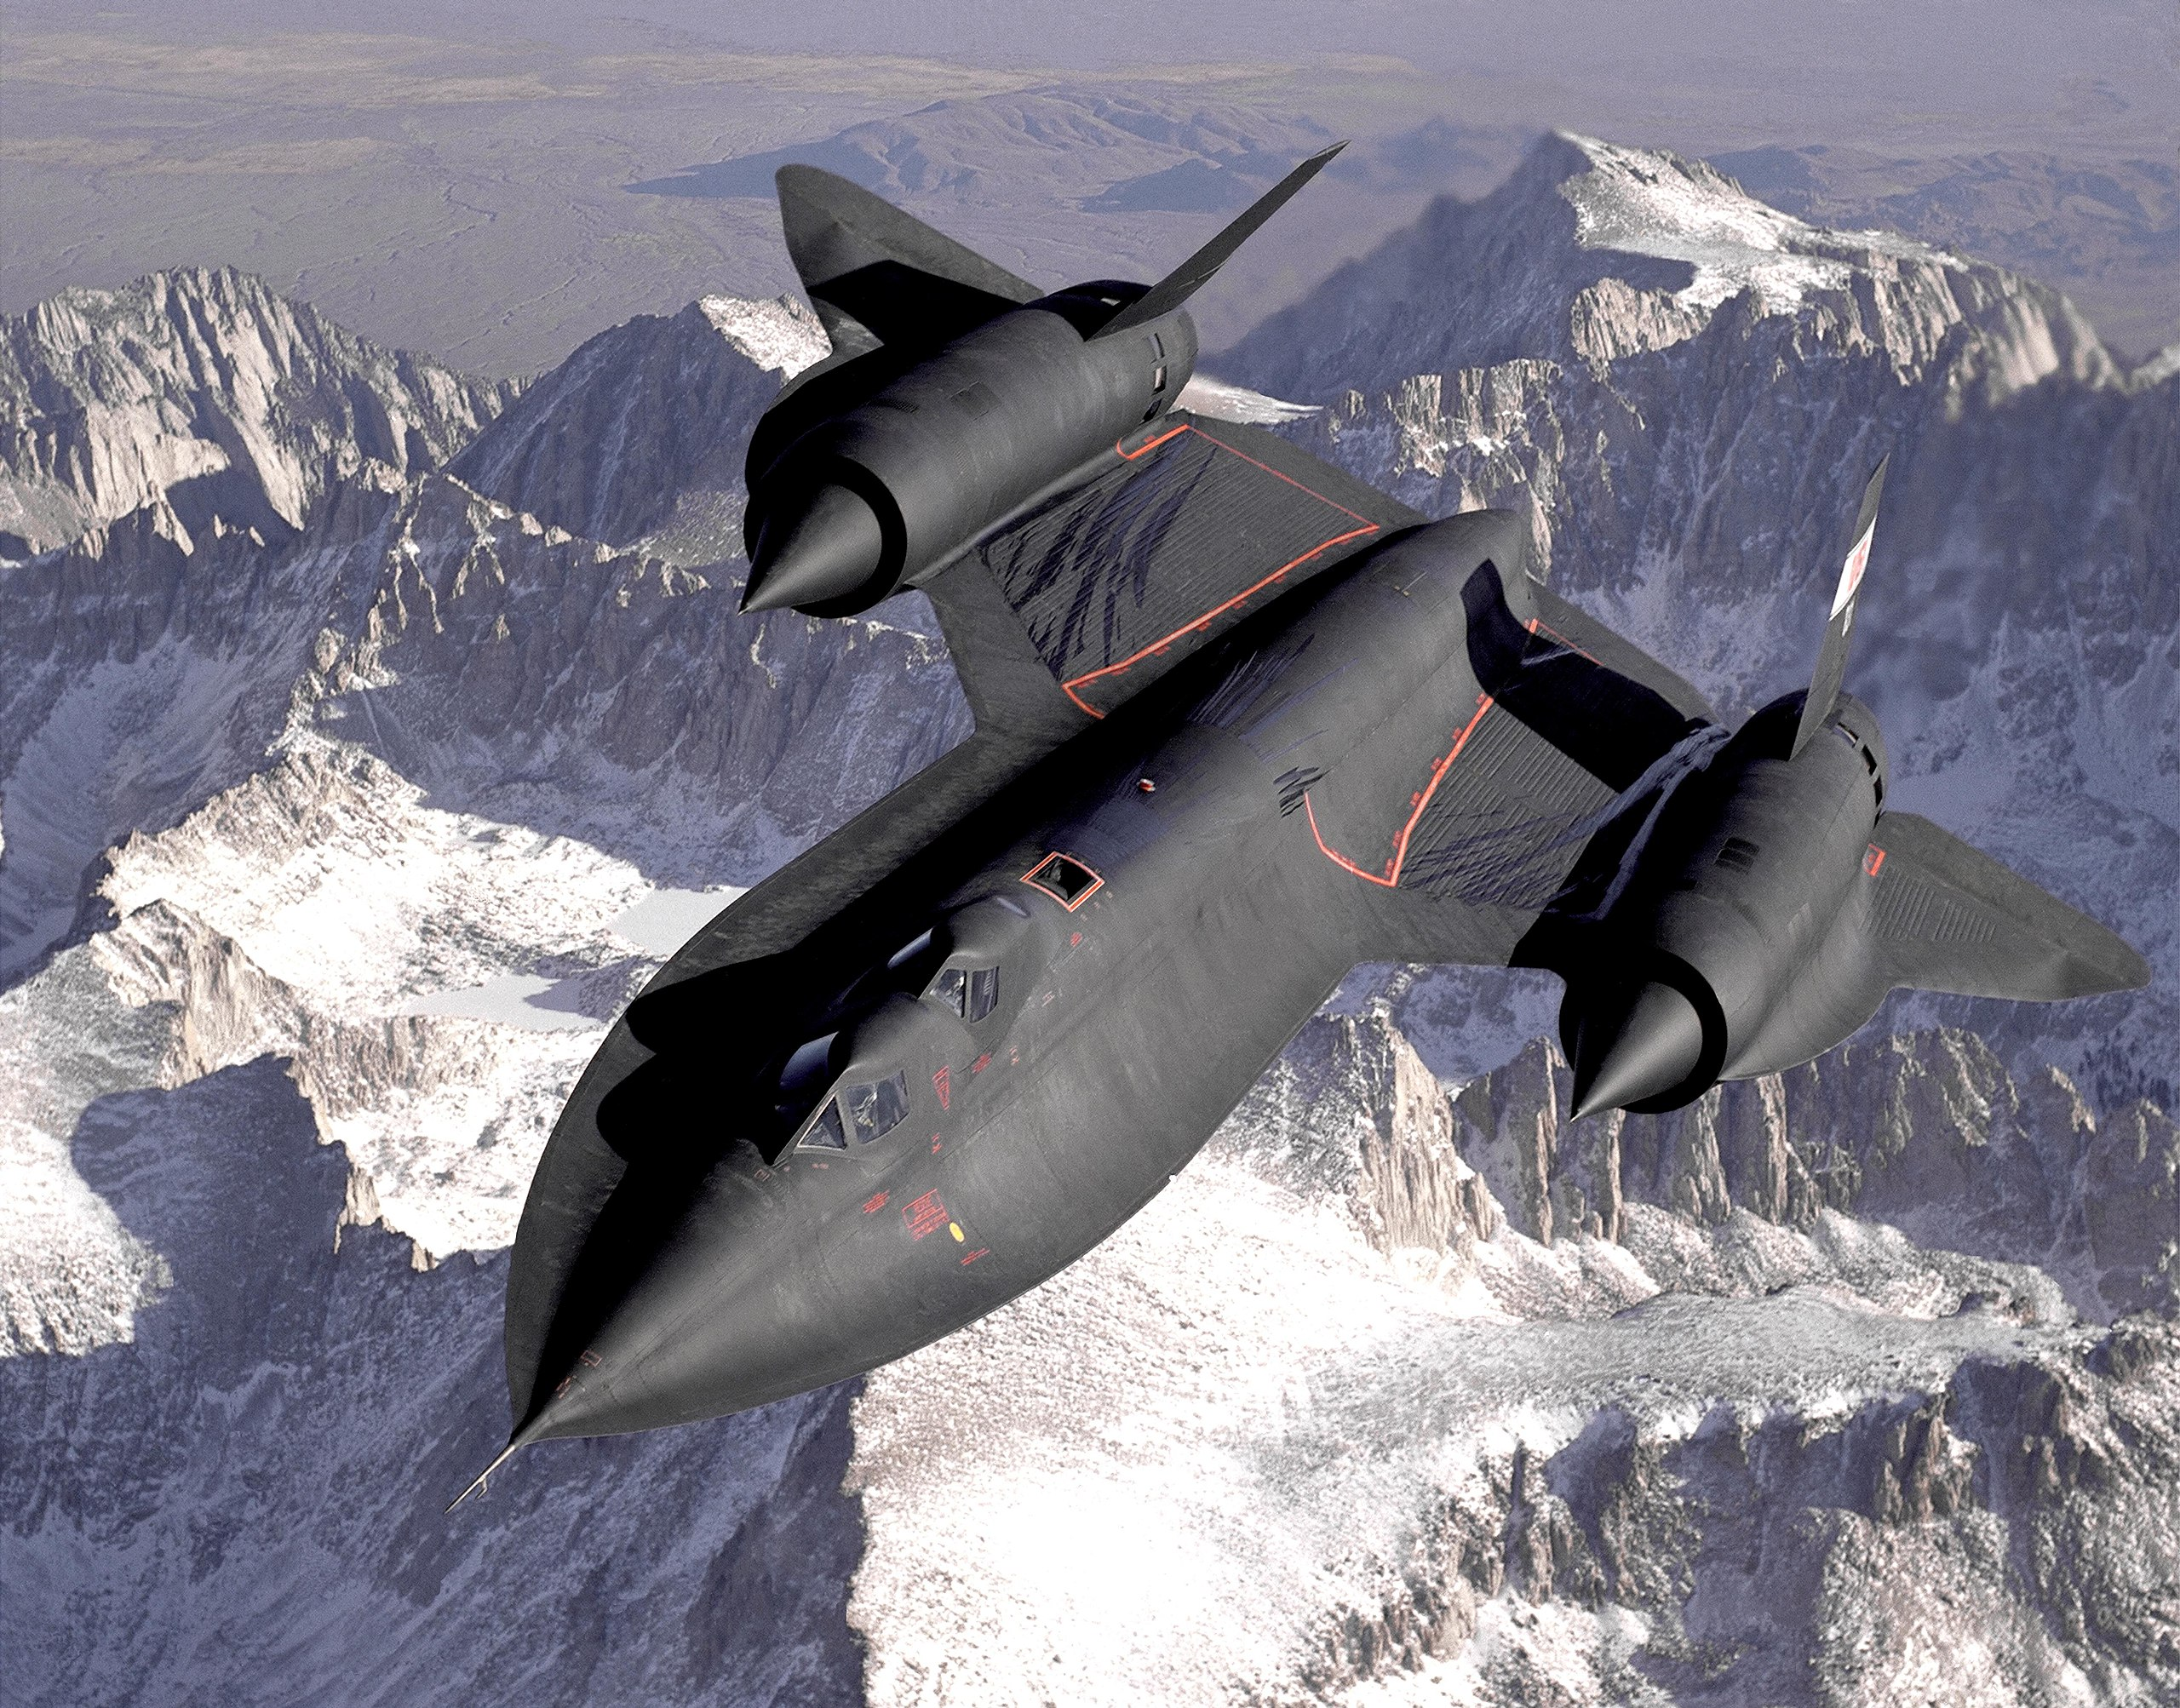
\includegraphics[width=0.8\textwidth]{images/blackbird.jpg}
\end{center}
\hfill SR-71B Blackbird. Photo Credit: USAF / Judson Brohmer
\end{changemargin}
\end{frame}

\begin{frame}
\frametitle{What is Fast?}

\Large
Program execution as completion of some number of items---things to do. 

We have two concepts:\\
\quad (1) items per unit time \\
\qquad \qquad (bandwidth---more is better)\\
\quad (2) time per item \\
\qquad \qquad (latency---less is better). 

Improving on either of these will make your program ``faster'' in some sense.

\end{frame}

\begin{frame}
\frametitle{Our Metrics}
\Large
In a way they are somewhat related. 

If we reduce the time per item from 5~s to 4~s, \\
it means an increase of 12 items per minute to 15 items per minute.

\qquad ...if the conditions are right. 

Hopefully we could improve both metrics; sometimes we'll have to pick one.



\end{frame}

\begin{frame}
\frametitle{Bandwidth}

\Large
This measures how much work can get 
done simultaneously.

Parallelization improves the number
of items per unit time. 

``Never underestimate the bandwidth of a station wagon full of tapes hurtling down the highway.''

\hfill --- Andrew S. Tanenbaum

\end{frame}




\begin{frame}
\frametitle{Latency}

\Large
This measures how much time it takes to do
any one particular task.

Also called response time.

It doesn't tend to get measured as often as bandwidth, but it's especially
important for tasks where people are involved. 

Google cares, which is why they provide the {\tt 8.8.8.8} DNS servers.



\end{frame}


\begin{frame}
\frametitle{Sadako and the Hundred Paper Airplanes}
\Large

 Say you need to make
100 paper airplanes.

What's the fastest way of doing this?

\begin{center}

\includegraphics[width=0.4\textwidth]{images/paper-airplane.png}
\end{center}

\end{frame}


\begin{frame}
\frametitle{Bandwidth vs Latency}
\Large

\begin{center}
\begin{tikzpicture}
  \draw (-4,0) -- (4,0) node[below right,xshift=-4em] {high latency};
  \draw (0,-1.5) -- (0,1.5) node[right] {high bandwidth};
\end{tikzpicture}
\end{center}

We will focus on completing the items,\\
not on transmitting information.

The above example makes the difference between bandwidth and latency clear.

\end{frame}


\begin{frame}
\frametitle{Improving Latency}
\Large

A good way of writing faster code is by improving single-threaded 
performance. 

There is a limit to how much you can
improve single-threaded performance.

Any improvements here
may also help with the parallelized version. 

On the other hand, faster
sequential algorithms may not parallelize as well. 


\end{frame}




\begin{frame}
\frametitle{Profiling}
\Large

You can't successfully make your code faster \\
if you don't know why it's slow. 

Intuition seems to often be
wrong here. 

Run your program with realistic workloads under a profiling tool.

``Don't guess; measure''.

\end{frame}


\begin{frame}
\frametitle{Exercise Time!}

\Large
Let's take a quick minute to visit \\
\begin{center}
\large
\vspace*{-4em}
\url{http://computers-are-fast.github.io/}
\end{center}

\end{frame}

\begin{frame}
\frametitle{Self Assessment}

\Large
Are the results surprising to you? 

Did you do really well or really badly? 

Chances are that you got some right and some wrong\ldots
and the ones that were wrong were not just a little wrong, but off by several orders of magnitude. 
\end{frame}

\begin{frame}
\frametitle{Trust, but Verify}
\Large
Moral of the story is: don't just guess at what the slow parts of your code are. 

It's okay to have a theory as a starting point, but test your theory.

\end{frame}

\begin{frame}
\Large
\frametitle{Do Less Work}

A surefire way to be faster is to omit unnecessary
work. 

Two (related) ways of omitting work are:\\
\quad (1) avoid calculating intermediate results that you don't actually need;\\
\quad (2) compute results to only the accuracy that you need in the final output.


\end{frame}

\begin{frame}
\frametitle{A Note About Logging}
\Large
Producing text output to a log file or to a console screen is surprisingly expensive for the computer. 

Sometimes one of the best ways to avoid unnecessary work is to spend less time logging and reporting. 

It might make debugging harder, \\
but code faster.

\end{frame}

\begin{frame}
\frametitle{Caching}

\Large
A hybrid between ``do less work'' and ``be smarter'' is caching. 

Store the results of expensive, side-effect-free, operation
(potentially I/O and computation) and reuse them as long as you
know that they are still valid. 

Caching is really important in certain situations.


\end{frame}




\begin{frame}
\frametitle{Be Prepared}

\Large
If you know something that the user is going to ask for in advance, you can have it at the ready to provide upon request. 

Example: users want an Excel export of statistics on customs declarations. 

Report generation takes a while, and it means a long wait. 
\end{frame}

\begin{frame}
\frametitle{Pre-compute the report}

\Large
Alternative: data pre-generated and stored in database (updated as necessary).

Then putting it into Excel is simple and the report is available quickly.


\end{frame}



\begin{frame}
\frametitle{Be Smarter}
\Large

You can also use a better algorithm. 

This is probably ``low hanging fruit'' and by the time it's time for P4P techniques this has already been done. 

But if your sorting algorithm is $\Theta(n^{3})$ and you can replace it with one that is $\Theta(n^{2})$, it's a tremendous improvement.

There may even be yet better algorithms out there.


\end{frame}



\begin{frame}
\frametitle{Aspects of Being Smarter}
\Large

An improved algorithm includes better asymptotic performance
as well as smarter data structures and smaller constant factors.


Compiler optimizations (which we'll discuss in this course) help with
getting smaller constant factors. 

We may also need to be aware of cache
and data locality/density issues.

\end{frame}



\begin{frame}
\frametitle{Checking out from the Library}
\Large
\begin{changemargin}{-1cm}
\begin{center}
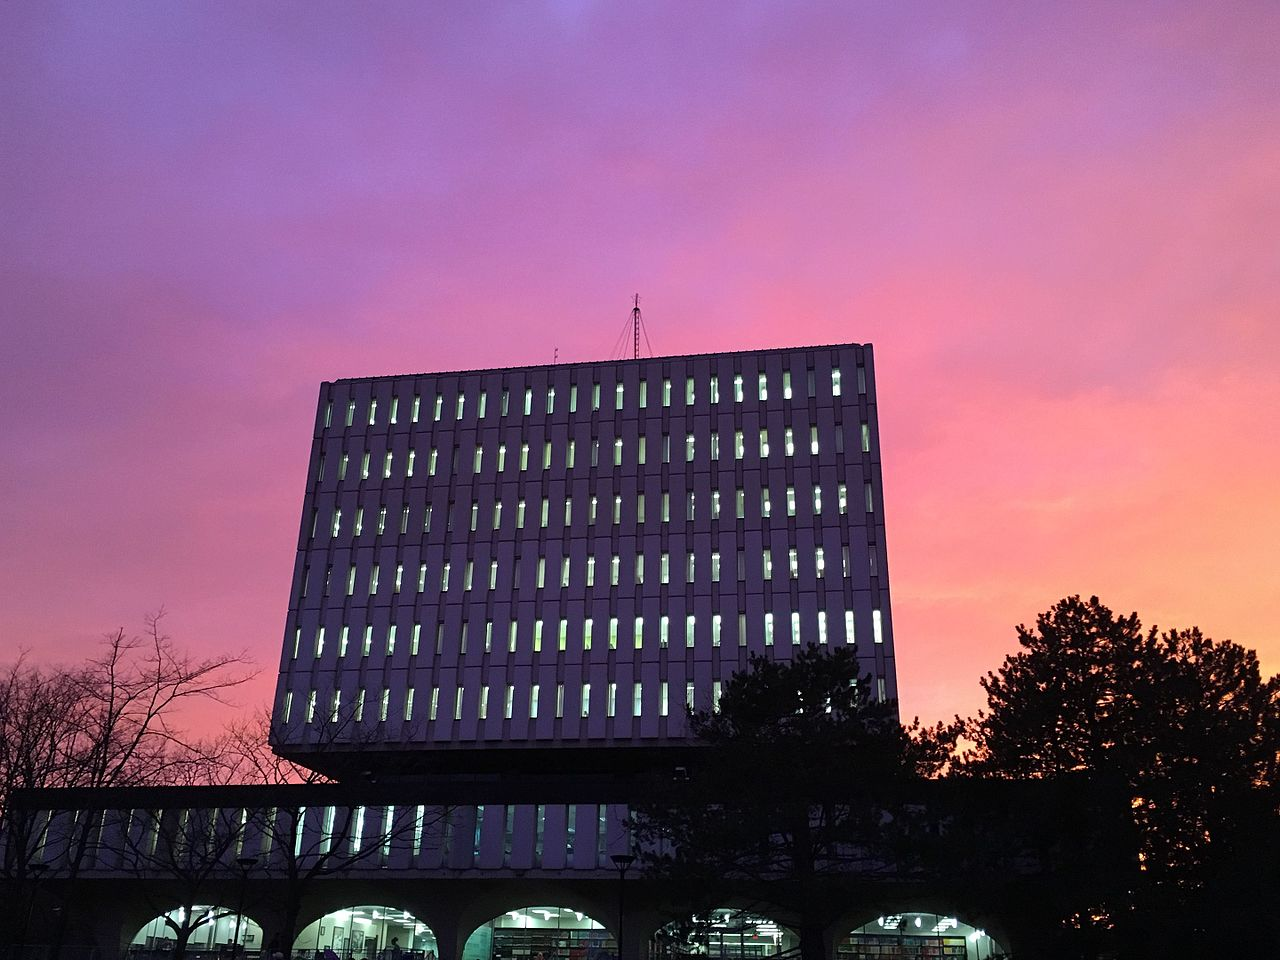
\includegraphics[width=.8\textwidth]{images/L01-Dana-Porter.jpg}
\end{center}
\end{changemargin}
{\hfill \small
Credit: Matt Polkiewicz via Wikimedia Commons, CC-SA-4.0}

Sometimes you can find this type of improvements in your choice of
libraries.

\end{frame}

\begin{frame}
\frametitle{When to Use the Library?}
\Large

Use a more specialized library which does the
task you need more quickly?
 
It's a hard decision sometimes. 

Libraries may be better and more reliable than the code you can write yourself. 

Or it might be better to write your own implementation that is optimized especially for your use case.

\end{frame}



\begin{frame}
\frametitle{Throw Money at the Problem}

\Large
Once upon a time, it was okay to write code with terrible performance---next year's CPUs would make it run acceptably. 

\begin{center}
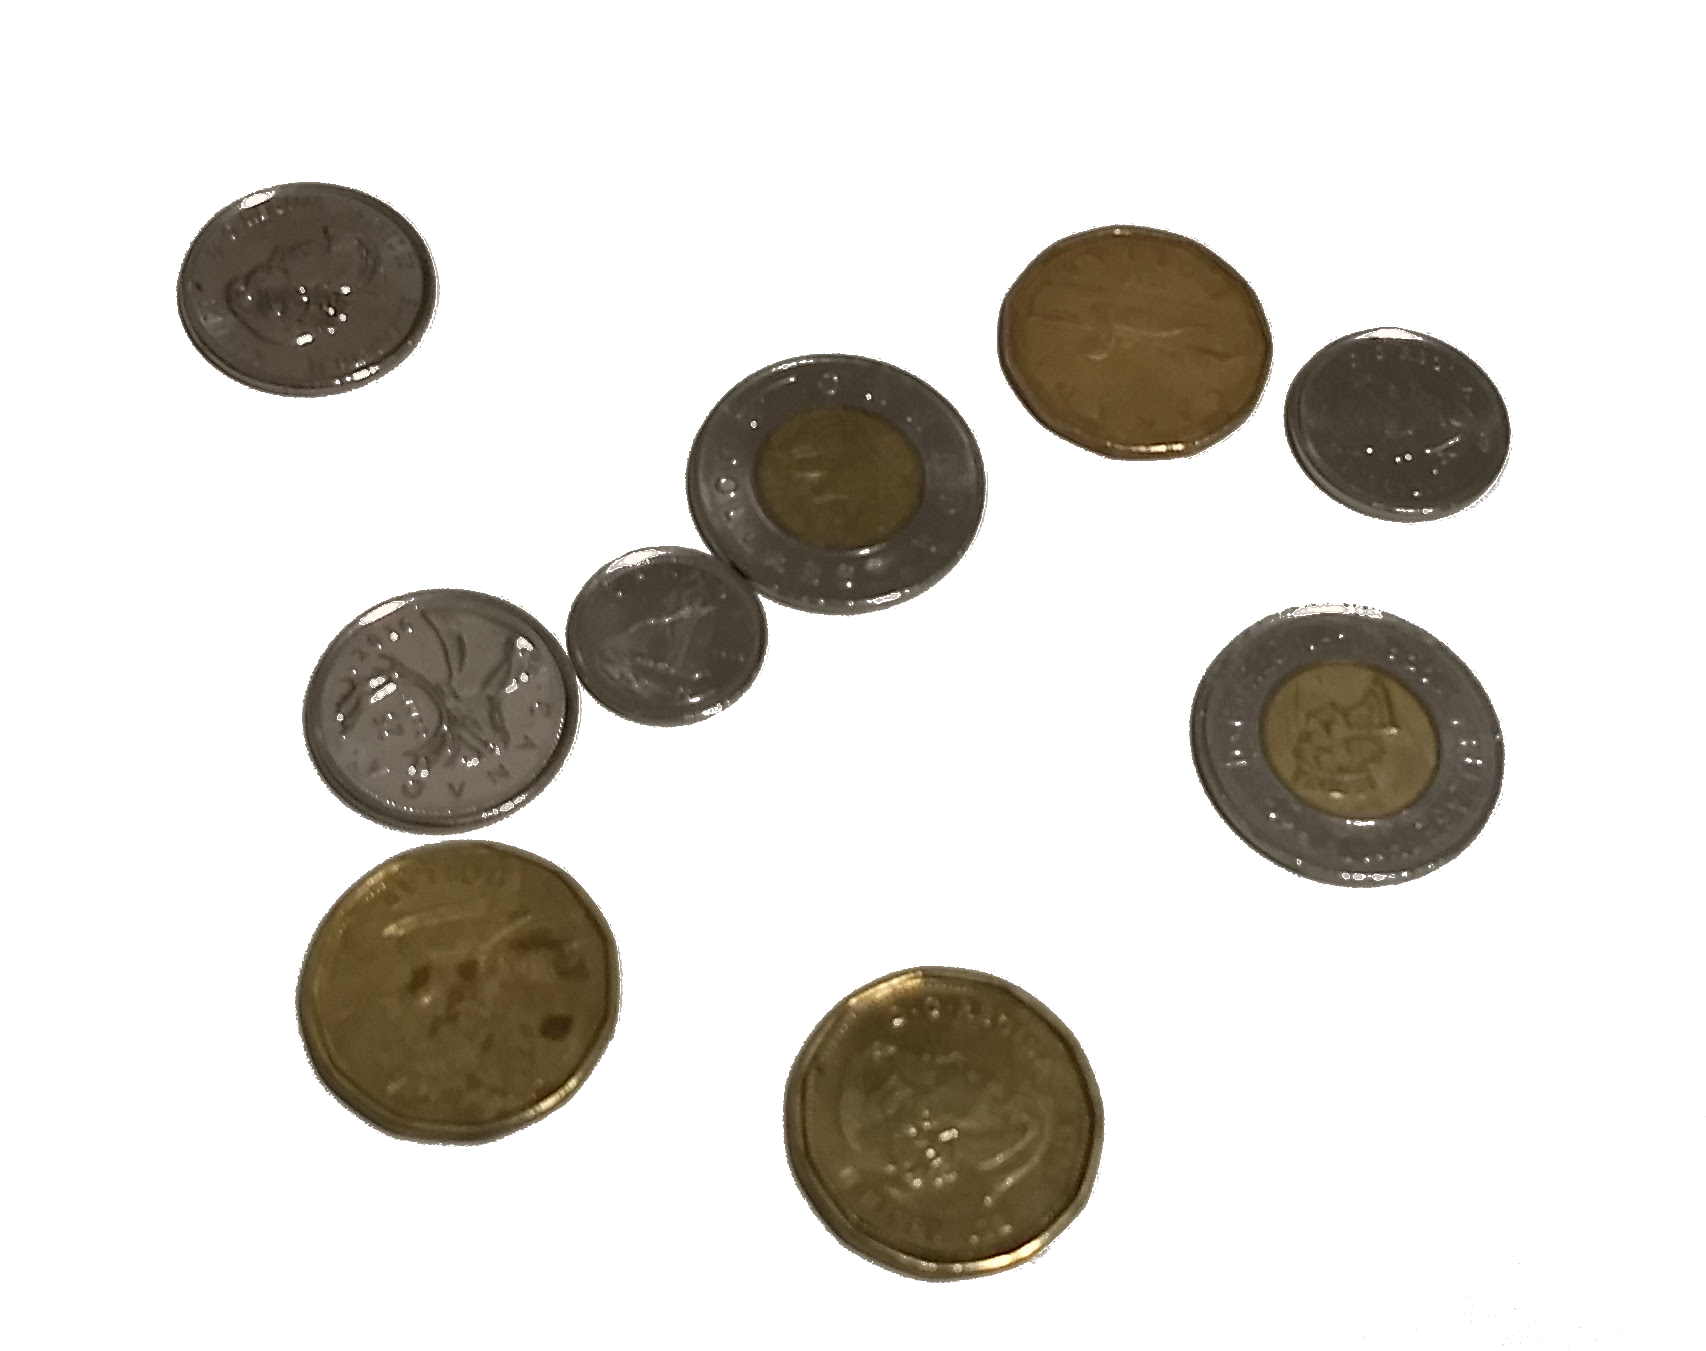
\includegraphics[width=.45\textwidth]{images/L01-money.png}
\end{center}
Spending a ton of time optimizing your code to run on today's processors was a waste of time. 

\end{frame}

\begin{frame}
\frametitle{No More Free Lunch}
\Large

Well, those days seem to be over.\\
CPUs are not getting much faster these days \\
(evolutionary, not revolutionary, change). 

\end{frame}



\begin{frame}
\frametitle{Spend Money to Save Money}

\Large
What if the CPU is not the limiting factor: your code might be I/O-bound.\\
\quad Buy some SSDs! 

You might be swapping out to disk, which kills performance .\\
\quad Add RAM. 
\end{frame}

\begin{frame}
\frametitle{Where should you spend money?}
\Large

Profiling is key here, to find out what the slow parts of execution are. 

Spending a few thousand dollars on better hardware is much cheaper than paying programmer time to optimize the code.


\end{frame}




\begin{frame}
\frametitle{MOV R1,R3}

\Large
What about outsmarting the compiler and writing assembly by hand? 

This tends to be a bad idea these days. 
\end{frame}

\begin{frame}
\frametitle{The Compiler Outsmarts You}

\Large
Compilers are going to be better at generating assembly than you are. 

CPUs may accept commands in x86 assembly (or your platform) but internally they don't operate on those commands directly. 

They rearrange and reinterpret and do their own thing. 

Still, it's important to understand what the compiler is doing, and why it can't optimize certain things (we'll discuss that), but you don't need to do it yourself.

\end{frame}



\begin{frame}
\frametitle{Anecdote Time}
\Large

``The report generation has been running for three hours; I think it's stuck.''

Nope, it reached a 30 minute time limit and got killed. 

How do I speed up this task to get it under the 30 minute time limit?

\end{frame}



\begin{frame}
\frametitle{Fly, My Pretties!}
\Large 
We can do more things at a time.

There are limits to how fast
you can do each thing. 
\end{frame}

\begin{frame}
\frametitle{Fly, My Pretties!}
\Large 
Often, it is easier to just throw more
resources at the problem: use a bunch of CPUs at the same time.

 We
will study how to effectively throw more resources at problems.

In general, parallelism improves bandwidth, but not latency.

Unfortunately, parallelism does complicate your life, as we'll see.



\end{frame}



\begin{frame}
\frametitle{Kinds of Parallelism}
\Large
Different problems are amenable to different sorts of parallelization. 

For instance, in a web server, we
can easily parallelize simultaneous requests. 

On the other hand, it's hard
to parallelize a linked list traversal. (Why?)



\end{frame}



\begin{frame}
\frametitle{Pipelining}
\Large

A key concept is pipelining. 

All modern CPUs do this,
but you can do it in your code too. 

Think of an assembly line: you can split
a task into a set of subtasks and execute these subtasks in parallel.


\end{frame}




\begin{frame}
\frametitle{Hardware}
\Large

To get parallelism, we need to have multiple instruction
streams executing simultaneously. 

We can do this by increasing the
number of CPUs: we can use multicore processors, SMP (symmetric
multiprocessor) systems, or a cluster or machines. 

We get different
communication latencies with each of these choices.

We can also use more exotic hardware, like graphics processing units
(GPUs).

\end{frame}



\begin{frame}
\frametitle{Mo' Parallelism, Mo' Problems}
\Large
You may have noticed that it is easier to do a project when it's just
you rather than being you and a team. 

The same applies to code.

\end{frame}



\begin{frame}
\frametitle{Exceptions}
\Large

Some domains are ``embarassingly parallel''; these problems
don't apply. 

It's easy to communicate the problem to all of the processors and to get the answer back.
 
The processors don't need to talk to each other to compute. 

The canonical
example is Monte Carlo integration.


\end{frame}



\begin{frame}
\frametitle{Limitations}
\Large
Here are some of the issues with parallel code.

First, a task can't start processing until it knows what it
is supposed to process. 

Coordination overhead is an issue. 

If the
problem lacks a succinct description, parallelization can be
difficult. 

Also, the task needs to combine its result with the other
tasks.

\end{frame}



\begin{frame}
\frametitle{Inherently Sequential Problems}
\Large

``Inherently sequential'' problems are an issue. 

In a sequential 
program, it's OK if one loop iteration depends on the result of the
previous iteration. 

However, such formulations \\
prohibit parallelizing
the loop. 

Sometimes we can find a parallelizable formulation of the loop,
but sometimes we haven't found one yet.

\end{frame}




\begin{frame}
\frametitle{Two Parts}
\Large

Finally, code often contains a sequential part and a parallelizable
part.  

If the sequential part dominates, then
executing the parallelizable part on infinite CPUs won't speed up the task as a whole. 

This is
known as Amdahl's Law, and we'll talk about this soon.


\end{frame}



\begin{frame}
\frametitle{To Avoid Complications\ldots}
\Large

 It's already quite difficult to make sure that
sequential programs work right. 

Making sure that a parallel program
works right is even more difficult.
\end{frame}

\begin{frame}
\frametitle{Beyond Total Orderings}
\Large
The key complication is that there is no longer a total ordering between
program events. 

Instead, you have a partial ordering:\\
\quad Some events $A$ are guaranteed to happen before other events $B$.\\
\quad Many events $X$  and $Y$ can occur in either the order $XY$ or $YX$.

\end{frame}



\begin{frame}
\frametitle{Races}
\Large

 A \alert{data race} occurs when two threads or processes both attempt to
simultaneously access the same data.

At least one of the accesses is a write. 

This can lead to nonsensical intermediate states becoming
visible.

Avoiding data races requires
coordination between the participants to ensure that intermediate
states never become visible (typically using locks). 


\end{frame}



\begin{frame}
\frametitle{Deadlock}
\Large

 \alert{Deadlock}
occurs when none of the threads or processes can make progress.

There is a cycle in the resource requests. 

To avoid a deadlock, the programmer needs to enforce an ordering in the locks.


\end{frame}



\begin{frame}
\frametitle{But Will it Scale?}
\Large

It gets worse. Performance is great, but it's not the only thing. 

We also care about \alert{scalability}: the trend of performance with increasing load. 

A program generally has a designed load (e.g., $x$ transactions per hour). 

A properly designed program will be able to meet this intended load. 

If the performance deteriorates rapidly with increasing load (that is, the number of operations to do), we say it is \alert{not scalable}.

\end{frame}



\begin{frame}
\frametitle{Scaling Up}
\Large

If we have a good program design,\\
it can be fixed. 

If we have a bad program design: \\
``rearranging deck chairs on the Titanic''.

Even the most scalable systems have their limits, of course, and while higher is better, nothing is infinite.

\end{frame}

%% \begin{frame}
%% \frametitle{Recap: The Roadmap}
%% Baseline understanding of hardware: architecture, caches, branch prediction.

%% Parallelize your program: threads, locking (but do it well!).

%% Speculation, single thread performance, OpenCL.

%% Profiling tools to find where and what to focus on next. 

%% Use multiple machines: such as with MPI, queueing theory.

%% \end{frame}

\begin{frame}[fragile]
\frametitle{Recap: The Roadmap}
\begin{tikzpicture}[remember picture, overlay]
\node[draw] (hw) at ([yshift=-3cm]current page.north) { \begin{tabular}{c}1. Grok the HW \\ (ECE 222++)\end{tabular}};

\node[draw] (par) at ([xshift=-1.5cm, yshift=-1.5cm]hw) { \begin{tabular}{c} 2. Parallelize code well.\\ (threads, locking) \end{tabular}};

\node[draw] (misc) at ([xshift=.5cm, yshift=-1.5cm]par) { \begin{tabular}{c} 3. Speculation, 1-thread perf, OpenCL \end{tabular}};

\node[draw] (prof) at ([xshift=3.5cm, yshift=-1.5cm]hw) { \begin{tabular}{c} 4. Profiling \\ (what's slow?) \end{tabular}};

\node[draw] (dist) at ([xshift=1.5cm, yshift=-1.5cm]misc) { \begin{tabular}{c} 5. Use many machines \\ (MPI, queueing theory) \end{tabular}};


%% Baseline understanding of hardware: architecture, caches, branch prediction.

%% Parallelize your program: threads, locking (but do it well!).

%% Speculation, single thread performance, OpenCL.

%% Profiling tools to find where and what to focus on next. 

%% Use multiple machines: such as with MPI, queueing theory.
\end{tikzpicture}

\end{frame}


\end{document}

